\question[10] En un teatro quieren construir escalones movibles que puedan
usarse para subir y bajar del escenario,
como los que aparecen en la figura \ref{fig:vol_area_01}.
Quieren que los escalones tengan suficiente espacio dentro para poder
almacenar objetos de utilería.
\textbf{¿Cuánto espacio hay dentro de los escalones?}\\
\textit{Escribe una respuesta exacta (no redondeada).}

\begin{minipage}{0.3\linewidth}
    \begin{figure}[H]
        \begin{center}
            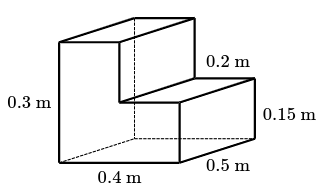
\includegraphics[width=1\textwidth]{../images/vol_area_01}
        \end{center}
        \caption{}
        \label{fig:vol_area_01}
    \end{figure}
\end{minipage}
\begin{minipage}{0.7\linewidth}
    \begin{solutionbox}{6cm}        El volumen de una figura irregular puede calcularse descomponiendo la figura en prismas rectangulares de largo $x$, ancho $y$ y altura $z$, cuyo volumen es:
        \begin{equation*}
            V = xyz
        \end{equation*}
        De la figura \ref{fig:vol_area_01} se sabe que $r=2$ y $h=5$, entonces
        \begin{equation*}
            \begin{split}
                V & = \pi r^2 h\\
                & = \pi (4)^2 (10)\\
                & = \pi (16) (10)\\
                & = 160\pi
            \end{split}
        \end{equation*}
    \end{solutionbox}
\end{minipage}